\chapter{Multi Layer Perceptron (MLP)}

\section{Difference between Machine Learning and Deep Learning}
The performance of machine learning algorithms heavily depends on the way we represent the data. These discrete pieces of information that we use as a proxy to model the complexity of the world are usually called features. Generally speaking, for a long time, these features have been handcrafted differently for each task at hand. However, traditional machine learning methods are inherently limited by this feature extraction process, since the quality of the final model strongly relies on the quality of the manually designed features.

In contrast, deep learning algorithms remove this limitation by simultaneously performing both feature extraction and learning the function that classifies (or predicts) the data within the same model. This means that the network itself learns the most suitable representations directly from raw data, without requiring handcrafted features. Moreover, in a deep neural network, it is not straightforward to pinpoint where feature extraction ends and classification begins, as both processes are deeply intertwined within the layered structure of the model.

\begin{figure}[H]
    \centering
    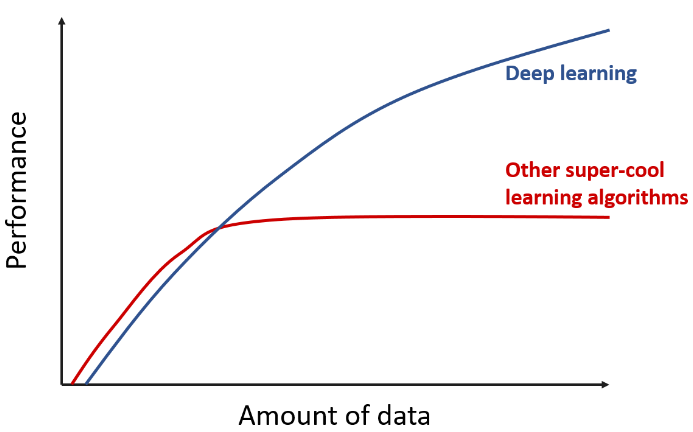
\includegraphics[width=0.5\textwidth]{images/size_matter.png}
    \caption{Why size matter}
    \label{fig:size_matter}
\end{figure}

\section{One step back: Linear classifier}
For the purpose of this lecture, we will stick to the task of image classification. 
Let’s assume we have a training dataset of $N$ images

\begin{equation}
x_i \in \mathbb{R}^D, \quad i = 1, \ldots, N
\end{equation}

that we want to classify into $K$ distinct classes. 
Thus, the training set is made of pairs

\begin{equation}
(x_i, y_i), \quad y_i \in \{1, \ldots, K\}
\end{equation}

Our goal is to define a function

\begin{equation}
f : \mathbb{R}^D \rightarrow \mathbb{R}^K
\end{equation}

that maps images to class scores.

As a real-world example, let’s take the CIFAR-10 dataset, which consists of 
$N = 60{,}000$ $32 \times 32$ RGB images belonging to 10 different classes. 

\begin{figure}[H]
    \centering
    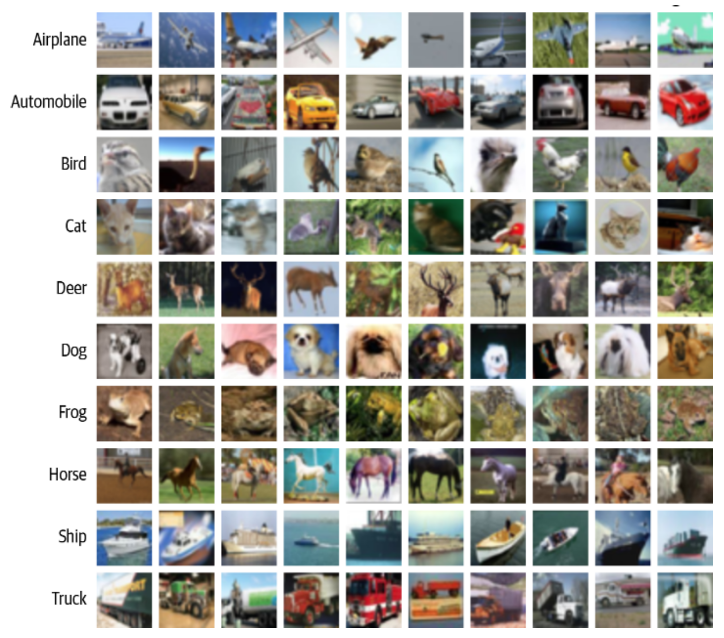
\includegraphics[width=0.5\textwidth]{images/cifrar_10.png}
    \caption{Why Cifrar-10 dataset}
    \label{fig:cifrar_10}
\end{figure}

Each image has dimensions $32 \times 32 \times 3$, and can therefore be represented as a column vector

\begin{equation}
x_i \in \mathbb{R}^{3072}
\end{equation}

We can now define a linear mapping:

\begin{equation}
f(x_i, W, b) = W x_i + b
\end{equation}

where the parameters are:

\begin{equation}
W \in \mathbb{R}^{10 \times 3072}, \quad b \in \mathbb{R}^{10}
\end{equation}

The role of the weight matrix is to learn how each pixel contributes to the class scores. 
The bias term, instead, is crucial because it allows us to \textbf{translate the decision boundaries} of the classes 
with respect to the same reference system. 
Without the bias, all class boundaries would be constrained to pass through the origin, 
which would unnecessarily limit the flexibility of the classifier.

Intuitively, our goal is to learn the parameters from the training data, when a new test image $x_i^{\text{test}}$ is presented to the model, the score of the correct class is higher that the scores of other classes-

\begin{figure}[H]
    \centering
    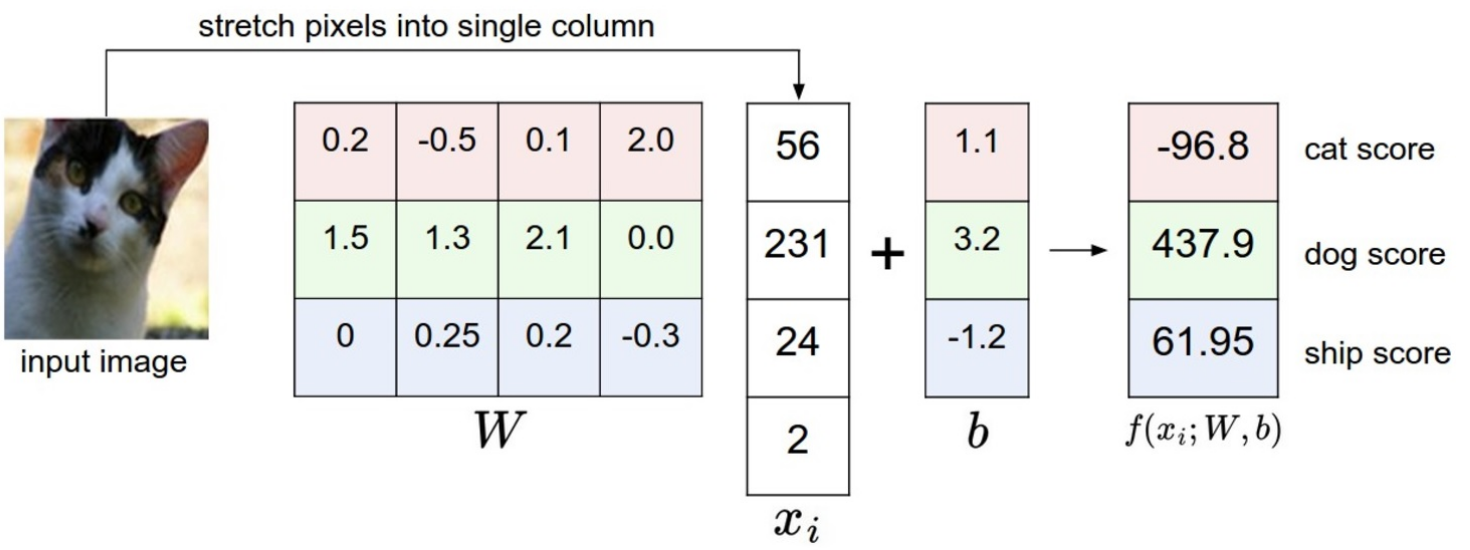
\includegraphics[width=0.8\textwidth]{images/linear_ex.png}
    \caption{Example of mapping an image to a score. For the sake of the visualization, here the image is assumed to have only 4 grayscale pixels.}
    \label{fig:linear_ex}
\end{figure}

\subsection{Logistic Regression}

If we add a sigmoid non-linearity to our linear mapping, we get a logistic regression classifier:

\begin{equation}
f(x_i, W, b) = \sigma(W x_i + b), \quad \text{where } \sigma(x) = \frac{1}{1 + e^{-x}}
\end{equation}

This model can be trained by optimizing the so-called \textit{binary cross-entropy loss}:

\begin{equation}
L(W, b) = - \frac{1}{m} \sum_{i=1}^{m} \Big( y_i \log(f_{x_i}) + (1 - y_i) \log(1 - f_{x_i}) \Big)
\end{equation}

Here, $m$ is the number of examples in the training set, and $f_{x_i}$ (with an abuse of notation) denotes $f(x_i, W, b)$.  

Let’s try to understand better the binary cross-entropy loss:

\begin{equation}
L(W, b) = - \frac{1}{m} \sum_{i=1}^{m} \Big( y_i \log(f_{x_i}) + (1 - y_i) \log(1 - f_{x_i}) \Big)
\end{equation}

Note that $y_i \in \{0, 1\}$, since this is a binary classification task.  

\begin{figure}[H]
    \centering
    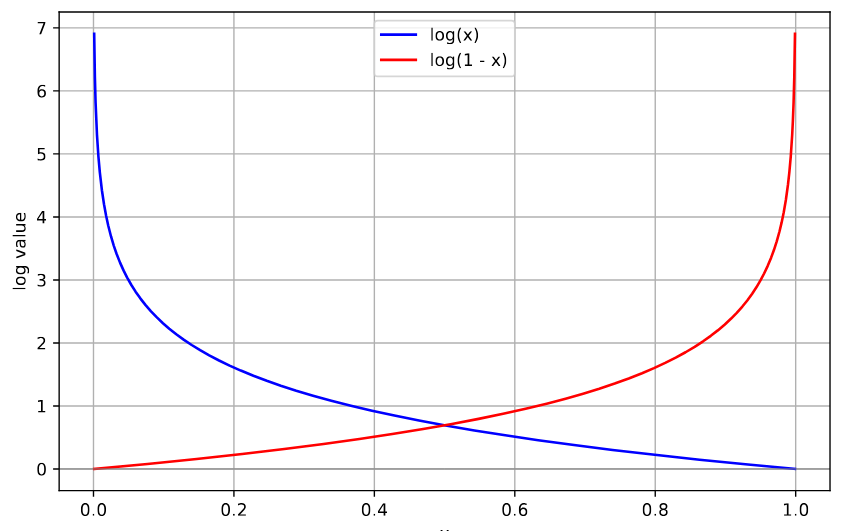
\includegraphics[width=0.5\textwidth]{images/log.png}
    \caption{log(x) and log(1-x) functions}
    \label{fig:log}
\end{figure}

The label $y_i$ act as a selector. For positive examples we penalize predictions close to zero. For negative examples we penalize predictions close to one.

\subsection{Softmax Classifier}
Softmax Classifier generalizes Logistic Regression to multi-class problems. We first define the softmax function:
\begin{equation}
\text{softmax}_j(z) = \frac{e^{z_j}}{\sum_{K} e^{z_j}}
\end{equation}

It takes a vector of arbitary real-valued scores and squashes it to a vector of values between zero and one that sum to one. Example:

\[
z =
\begin{bmatrix}
1.2 \\
5.1 \\
2.7
\end{bmatrix}, 
\quad
\text{softmax}(z) =
\begin{bmatrix}
0.018 \\
0.90 \\
0.08
\end{bmatrix}
\]

\textbf{Note:} ThSoftmax transforms the scores into probabilities that sum to 1, but the relative ratios of the original scores are distorted because of the exponential, which emphasizes larger values and suppresses smaller ones.

In the softmax classifier, the scores of the linear function mapping 

\begin{equation}
f(x_i, W) = W x_i
\end{equation}

are interpreted as unnormalized log probabilities. To train the classifier we optimize the cross-entropy loss:

\begin{equation}
L = \sum_i y^{\text{true}}_i \log(y^{\text{pred}}_i)
\end{equation}

where $y^{\text{true}}_i$ is the ground truth output distribution and $y^{\text{pred}}_i$ is the predicted output distribution. 

In practice, $y^{\text{true}}_i$ is a one-hot vector selecting the output of the correct label. 

\textbf{Notice:} the softmax classifier has the appealing property to produce an easy-to-interpret output, 
that is, the normalized score confidence for each class.

\section{Modelling a Neuron}

Neural Networks are a mathematical model \textbf{coarsely} inspired by the way our own brain works

\begin{figure}[H]
    \centering
    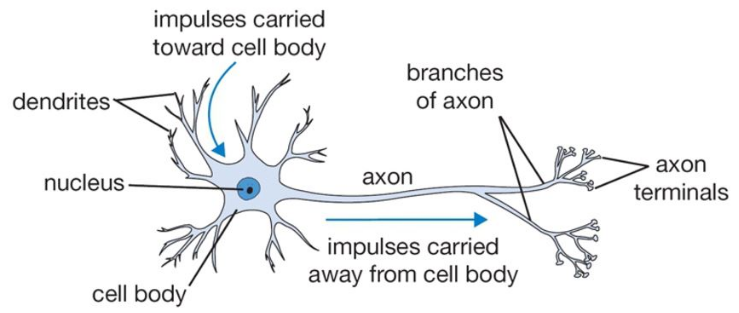
\includegraphics[width=0.6\textwidth]{images/neuron.png}
    \caption{Neuron model}
    \label{fig:neuron}
\end{figure}

Neurons are the basic computational unit of our brain. Approximately 86 billion neurons can
be found in the human nervous system and they are connected with approximately $10^14$-$10^15$
\textbf{synapses}. Each neuron receives input signals from its \textbf{dendrites} and produces output signals
along its (single) \textbf{axon}. The axon eventually branches out and connects via synapses to
dendrites of other neurons.

More formally, we can model a single \textbf{neuron} as follows:

\begin{figure}[H]
    \centering
    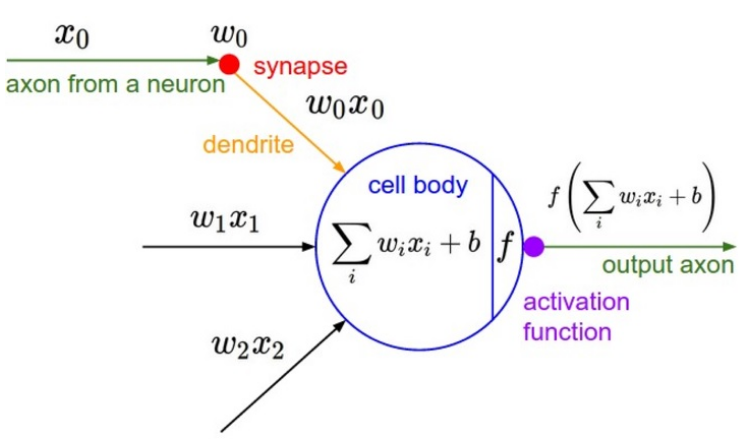
\includegraphics[width=0.5\textwidth]{images/artificial_neuron.png}
    \caption{Artificial Neuron model}
    \label{fig:artificial_neuron}
\end{figure}

Each neuron can have multiple inputs. The neuron's output is the dot product between the inputs and its weughts, plus the bias; then an activation function is applied, generally a non-linearity.

It's easy to see that a single neuron can be used to implement a binary classifier. Indeed, when loss is applied to the output of the neuron, we can optimize a \textbf{binary Softmax classifier} (a.k.a. Logistic Regression).


\subsection{Neuron Activation Functions}

Activation functions are non-linear functions computed on the output of each neuron. 
Commonly used activations include \textbf{sigmoid}, \textbf{tanh}, and \textbf{ReLU}, 
although more complex activations also exist.

\subsubsection{Sigmoid}
The sigmoid activation function is defined as:
\begin{equation}
\sigma(x) = \frac{1}{1 + e^{-x}}
\end{equation}

\begin{compactitemize}
  \item Squashes any real-valued input into the range $[0, 1]$.
  \item Historically widely used, but now less common.
  \item \textbf{Drawbacks:}
  \begin{compactitemize}
    \item Saturates for large positive or negative values, leading to vanishing gradients.
    \item Output is not zero-centered, which can slow down convergence.
  \end{compactitemize}
\end{compactitemize}

\begin{figure}[H]
    \centering
    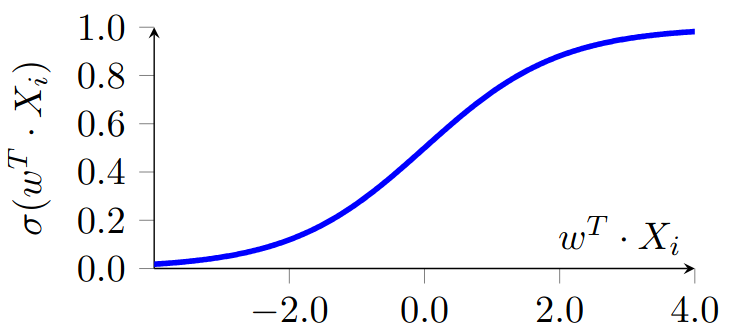
\includegraphics[width=0.5\textwidth]{images/sigmoid.png}
    \caption{Sigmoid activation function}
    \label{fig:sigmoid}
\end{figure}

\subsubsection{Tanh}
The tanh activation function is a scaled sigmoid:
\begin{equation}
\tanh(x) = 2\sigma(x) - 1
\end{equation}

\begin{compactitemize}
  \item Squashes input to the range $[-1, 1]$.
  \item Output is zero-centered.
  \item \textbf{Drawback:} activation can still saturate for large inputs, causing vanishing gradients.
\end{compactitemize}


\begin{figure}[H]
    \centering
    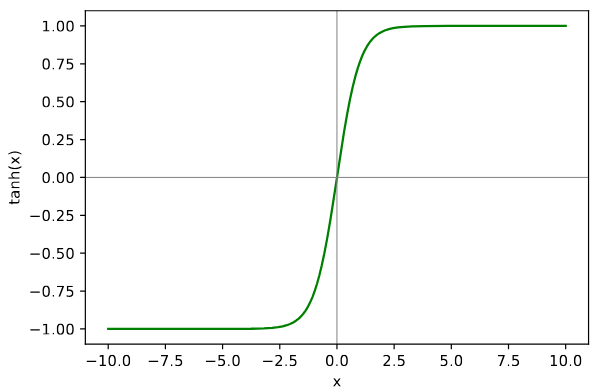
\includegraphics[width=0.5\textwidth]{images/tanh.png}
    \caption{Tanh activation function}
    \label{fig:tanh}
\end{figure}

\subsubsection{ReLU (Rectified Linear Unit)}
The ReLU activation function is defined as:
\begin{equation}
\text{ReLU}(x) = \max(0, x)
\end{equation}

\begin{compactitemize}
  \item Accelerates convergence of SGD compared to sigmoid/tanh.
  \item Simple to implement: threshold at 0, no expensive exponential computations.
  \item \textbf{Solves positive saturation:}
  \begin{compactitemize}
    \item For $x>0$, gradient is 1 → no vanishing gradient for positive values.
    \item For $x\le0$, gradient is 0 → negative part is inactive.
  \end{compactitemize}
\end{compactitemize}


\begin{figure}[H]
    \centering
    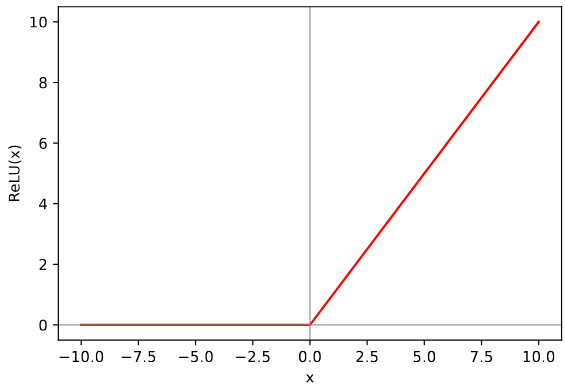
\includegraphics[width=0.5\textwidth]{images/relu.png}
    \caption{ReLU activation function}
    \label{fig:relu}
\end{figure}

\subsubsection{Why Non-linear Activations?}
\begin{compactitemize}
  \item Composition of linear functions is still linear.
  \item Without nonlinearities, a neural network reduces to a single linear transformation:
  \begin{equation}
  f(x) = \phi(W_2 \phi(W_1 x)) \quad \text{with nonlinear activation } \phi
  \end{equation}
  \item Removing the nonlinearities:
  \begin{equation}
  f(x) = W_2 W_1 x = W x
  \end{equation}
  \item Clearly still linear, so no hierarchical feature learning would occur.
\end{compactitemize}

\section{Neural Networks}
When we connect an ensemble of neurons in a graph is when the magic happens and we get an actual Multilayer Perceptron (MLP)
Neural Networks are arranged in layers, with one input layer, one output layer, and N hidden layers in the middle.

\begin{figure}[H]
    \centering
    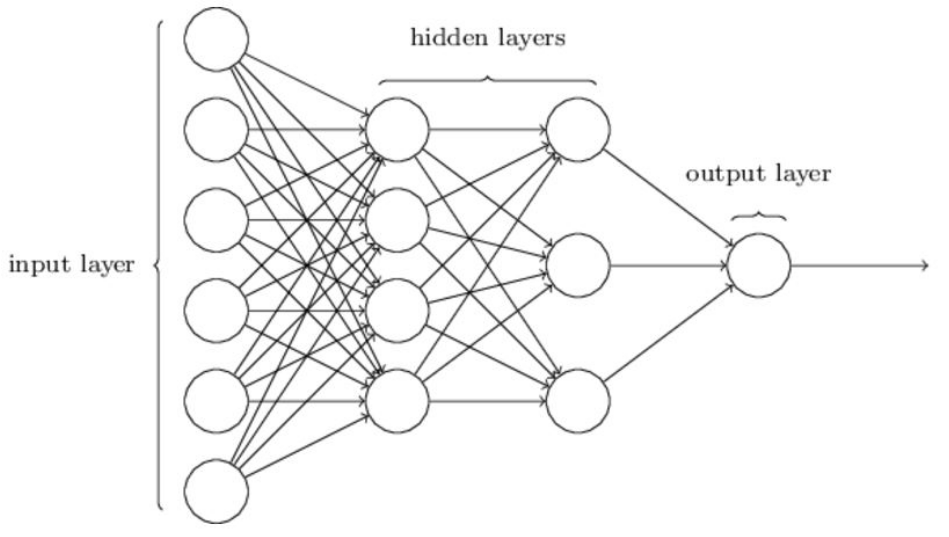
\includegraphics[width=0.4\textwidth]{images/NN.png}
    \caption{A simple Neural Network with 2 hidden layers}
    \label{fig:NN}
\end{figure}

The 4-layer network previously depicted can be expressed as:

\begin{equation}
\text{out} = \phi \Big( W_3 \, \phi \big( W_2 \, \phi ( W_1 x ) \big) \Big)
\end{equation}

where:

\begin{compactitemize}
  \item $\phi$ is the activation function.
  \item $x \in \mathbb{R}^6$ is the input.
  \item $W_1 \in \mathbb{R}^{4 \times 6}$ are the weights of the first layer.
  \item $W_2 \in \mathbb{R}^{4 \times 3}$ are the weights of the second layer.
  \item $W_3 \in \mathbb{R}^{1 \times 3}$ are the weights of the third layer.
\end{compactitemize}

\noindent
\textbf{Note:} To ease notation, biases have been incorporated into the weight matrices $W$.

\subsection{Forward propagation}
Forward propagation is the process of computing the output of the neural network given an input.
It involves passing the input through each layer of the network, applying the weights, biases, and activation functions at each step.

\begin{figure}[H]
    \centering
    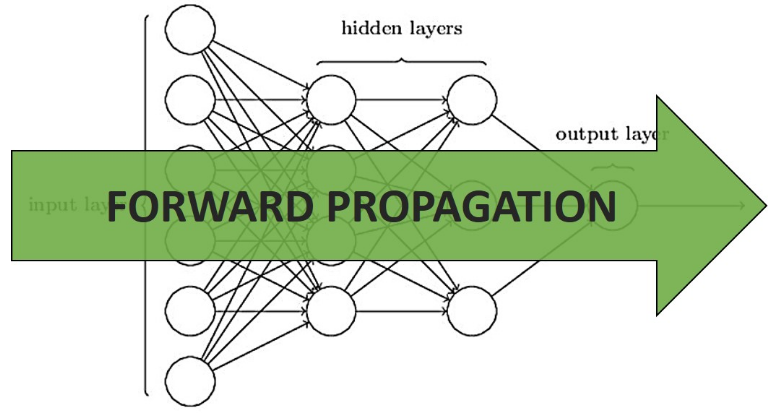
\includegraphics[width=0.4\textwidth]{images/forward.png}
    \caption{Forward propagation in a Neural Network}
    \label{fig:forward}
\end{figure}

\subsection{Representational Power}

It has been shown that any continuous function $f(x)$ can be approximated at arbitrary precision $\epsilon > 0$ by a neural network $g(x)$ with at least one hidden layer:

\begin{equation}
\forall x, \quad |f(x) - g(x)| < \epsilon
\end{equation}

\begin{compactitemize}
  \item Neural networks with at least one hidden layer are referred to as \textbf{universal approximators}.
  \item In practice, networks with more layers often outperform 2-layer networks, 
        even though their representational power is theoretically the same.
\end{compactitemize}

\subsection{Setting Hyperparameters}

The number of layers in the network, as well as the number of neurons in each layer, are 
so-called \textbf{hyperparameters} of the architecture. Keep in mind:

\begin{compactitemize}
  \item The bigger the size and the number of layers, the more the capacity of the network 
        increases. This is beneficial because the space of representable functions grows.
  \item Bigger networks without proper regularization are much more prone to 
        overfitting the training data, which is undesirable.
\end{compactitemize}


In practice, usually networks are made
as big as allowed by the computational
budget.
Then overfitting is prevented through
proper regularization techniques
(e.g. dropout, weight decay, input
noise, etc.).

\begin{figure}[H]
    \centering
    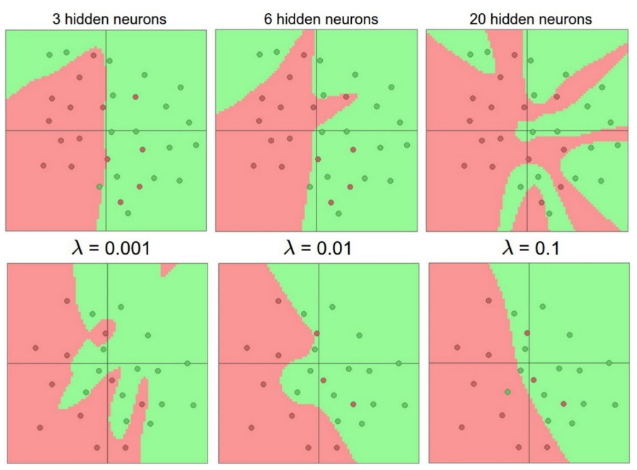
\includegraphics[width=0.5\textwidth]{images/overF.png}
    \caption{Trying different hyperparameters}
    \label{fig:overF}
\end{figure}




